
\documentclass{tufte-handout}
\usepackage[T1]{fontenc}
\usepackage{babel}



\title[Ex.5]{Assignment 5 Educational activity - Reflection Report}

\author{Helena Rasche}
\date{2022-02-02}

\usepackage{graphicx} % allow embedded images
  \setkeys{Gin}{width=\linewidth,totalheight=\textheight,keepaspectratio}
  \graphicspath{{graphics/}} % set of paths to search for images
\usepackage{amsmath}  % extended mathematics
\usepackage{booktabs} % book-quality tables
\usepackage{pdfpages}
\usepackage{units}    % non-stacked fractions and better unit spacing
\usepackage{multicol} % multiple column layout facilities
\usepackage{lipsum}   % filler text
\usepackage{fancyvrb} % extended verbatim environments
  \fvset{fontsize=\normalsize}% default font size for fancy-verbatim environments

% Standardize command font styles and environments
\newcommand{\doccmd}[1]{\texttt{\textbackslash#1}}% command name -- adds backslash automatically
\newcommand{\docopt}[1]{\ensuremath{\langle}\textrm{\textit{#1}}\ensuremath{\rangle}}% optional command argument
\newcommand{\docarg}[1]{\textrm{\textit{#1}}}% (required) command argument
\newcommand{\docenv}[1]{\textsf{#1}}% environment name
\newcommand{\docpkg}[1]{\texttt{#1}}% package name
\newcommand{\doccls}[1]{\texttt{#1}}% document class name
\newcommand{\docclsopt}[1]{\texttt{#1}}% document class option name
\newenvironment{docspec}{\begin{quote}\noindent}{\end{quote}}% command specification environment

%%%%%%%%%%%%%%%%%%%%%%%%%%%%%%
%%% START JoST ADDITIONS %%%%%
%%%%%%%%%%%%%%%%%%%%%%%%%%%%%%

\usepackage{comment}
\usepackage{latexsym}
\usepackage[utf8]{inputenc}
%\usepackage{csquotes}
\usepackage{longtable}
\usepackage{cancel}
\usepackage{multirow}
\usepackage{amsmath}
\usepackage{array}
\usepackage{tikz}
\usetikzlibrary{arrows,matrix,positioning,fit,external,calc,tikzmark,arrows.meta,backgrounds}
\usepackage{tikz-network}
\usepackage{tikzpagenodes}
\usepackage{eso-pic}
%\tikzexternalize[prefix=tikz/]
%\usepackage{siunitx}
\usepackage{verbatim}
\usepackage[utf8]{inputenc}
\usepackage{blindtext}
\usepackage{xspace}
\usepackage{hologo}
\usepackage{tabularx}
\usepackage{amsfonts}
\usepackage{amssymb}
\usepackage{mathtools}
\usepackage{fdsymbol}
\usepackage{etex}
\usepackage{graphicx}
\usepackage{stackengine}
\stackMath




\newcolumntype{P}[1]{>{\centering\arraybackslash}p{#1}}
\newcolumntype{M}[1]{>{\centering\arraybackslash}m{#1}}
\makeatletter
\tikzset{
  prefix after node/.style={
    prefix after command={\pgfextra{#1}}
  },
  /semifill/ang/.store in=\semi@ang,
  /semifill/ang=0,
  semifill/.style={
    circle, draw,
    prefix after node={
      \typeout{aaa \semi@ang}
      \let\nodename\tikz@last@fig@name
      \fill[/semifill/.cd, /semifill/.search also={/tikz}, #1]
        let \p1 = (\nodename.north), \p2 = (\nodename.center) in
        let \n1 = {\y1 - \y2} in
        (\nodename.\semi@ang) arc [radius=\n1, start angle=\semi@ang, delta angle=180];
    },
  }
}
\makeatother
%\numberwithin{equation}{section}

\makeatletter
\newcommand{\lrarrow}{\mathrel{\mathpalette\lrarrow@\relax}}
\newcommand{\lrarrow@}[2]{%
  \vcenter{\hbox{\ooalign{%
    $\m@th#1\mkern6mu\rightarrow$\cr
    \noalign{\vskip1pt}
    $\m@th#1\leftarrow\mkern6mu$\cr
  }}}%
}
\makeatother

\newcommand\xtab[1][1cm]{\hspace*{#1}} % create \xtab


\newcolumntype{L}[1]{>{\raggedright\let\newline\\\arraybackslash\hspace{0pt}}m{#1}}
\newcolumntype{C}[1]{>{\centering\let\newline\\\arraybackslash\hspace{0pt}}m{#1}}
\newcolumntype{R}[1]{>{\raggedleft\let\newline\\\arraybackslash\hspace{0pt}}m{#1}}

\extrafloats{100}



\begin{document}

%%%%%%%%%%% Header and Footer %%%%%%%%%%%%%%%%%%
\fancyfoot[CE,CO]{\flushright 
\includegraphics[width=3cm]{../avans.jpg}}
\fancyhead[CE,CO]{\flushleft \smallcaps{\today}}

\maketitle % this prints the handout title, author, and date

%%%%%%%%%%% Start Author Section %%%%%%%%%%%%%%%%%%
Helena Rasche\textsuperscript{a,b}\marginnote{\\\textsuperscript{a}{\scriptsize ATGM, Avans Hogeschool, Breda}\\\textsuperscript{b}{\scriptsize Dept Pathology, Erasmus Medical Center}}
%%%%%%%%%%% End Author Section %%%%%%%%%%%%%%%%%%

\begin{abstract}
\noindent
After reviewing the reports from both Chen and Titia I've consolidated a
couple of key situations which I would like to address, namely the lack
of good pre- and post-class summaries and excessive apologising when a
missing course component was discovered.
\end{abstract}
\noindent\rule{5in}{0.4pt}



\hypertarget{situation-summaries}{%
\section{Situation: Summaries}\label{situation-summaries}}

The start of the class featured a slide deck I'd created for the express
purpose of introducing the topic to the audience. This included a couple
bullet points of what we would cover, but it wasn't called out as a
lesson plan, and it didn't include learning objectives. This should have
been included as it would help learners identify the lesson contents and
schedule and mentally prepare for the day.

\hypertarget{looking-back}{%
\subsection{Looking Back}\label{looking-back}}

In an ideal lesson, these aspects would be covered sufficiently, and
perhaps even I would have a checklist to go through before a lesson to
ensure the presence of key components. However, I need to balance my
perfectionism in this case, with the negative self talk that can result,
and be measured in my evaluation of the situation, i.e.~was it
significant enough to warrant stress. In my ideal, every class is up to
my standard of organisation because that's what I expect from others,
and organisation is something I value quite highly.

\hypertarget{awareness}{%
\subsection{Awareness}\label{awareness}}

This feels like a process failure to me, it was such a trivial part of
the lesson to include that missing it feels like a significant oversight
of something quite basic and easy to check for. By not being more
careful, I miss the ``low hanging fruit'' of lesson preparation, I feel
that I'm limiting my students in their education.

\hypertarget{alternatives}{%
\subsection{Alternatives}\label{alternatives}}

A course day ``checklist'' I think would be an extremely valuable tool
for me to develop for myself here. I use checklists in many other
contexts to ensure I'm well prepared, this would be an ideal tool to
leverage in the teaching context as well. It gives me an adaptable,
interactive tool to make sure that all necessary elements are part of
the day's plan. The primary disadvantage is ensuring that it's used
consistently across lessons, a problem which will need to be explored
during a trial.

\hypertarget{trials}{%
\subsection{Trials}\label{trials}}

Before my next course, I plan to make a checklist and try going through
it to see if it helps me achieve my desired level of preparedness and
organisation for my courses. I want to try that out as a tool for
ensuring lessons meet my standards and are useful to the students. I
need to be careful that it actually gets used regularly, and I find a
good way to integrate it in my workflow, maybe via regular calendar
reminders.

\hypertarget{situation-apologies}{%
\section{Situation: Apologies}\label{situation-apologies}}

During the start of the course, students needed to connect to a web
service only available within the Avans network. EduVPN allows access to
this service, but it was not included in the instructions despite that
it should have been caught during review. I apologised repeatedly for
this mistake since I felt responsible for missing it. In the end one of
the TOAs directed them through installing and it was fine.

In this case an additional bit of information was not made public - that
the lesson had not been on my calendar, it was officially assigned to a
colleague, and I was not told I'd be teaching until the day before. I
wrote the materials over 6 hours of testing and re-testing, but it did
not have time to be reviewed by any colleagues before the lesson.

\hypertarget{looking-back-1}{%
\subsection{Looking Back}\label{looking-back-1}}

I have high ideals for the success of lessons and this failure gives me
strong negative feelings which puts me on the wrong footing at the start
of a lesson. I value proper prior preparation.

\hypertarget{awareness-1}{%
\subsection{Awareness}\label{awareness-1}}

Even though there were clear process failures leading up to this point,
the excessive apologies were my own responsibility and could have been
avoided, I don't need to take responsibility for group failures like
that.

Especially when I'm able to handle similar technological failures and
work around those (e.g.~when my cocalc stopped loading temporarily), it
is remarkable that I feel so much responsibility for missing this
section of the materials.

\hypertarget{alternatives-1}{%
\subsection{Alternatives}\label{alternatives-1}}

I saw some great examples from Titia during her courses, she was a
really good role model here by acknowledging the issue without taking
responsibility or apologising excessively. Even once is enough and then
moving on to the resolution of the issue. The students know issues
happen and don't care.

\hypertarget{trials-1}{%
\subsection{Trials}\label{trials-1}}

While I don't desire to intentionally introduce a failure to force me to
practice this situation, I at least know I should work on my self
confidence with handling these teaching failures.


\bibliography{jost-bib}
\bibliographystyle{plainnat}


\clearpage
\addcontentsline{toc}{section}{Chen for Helena}
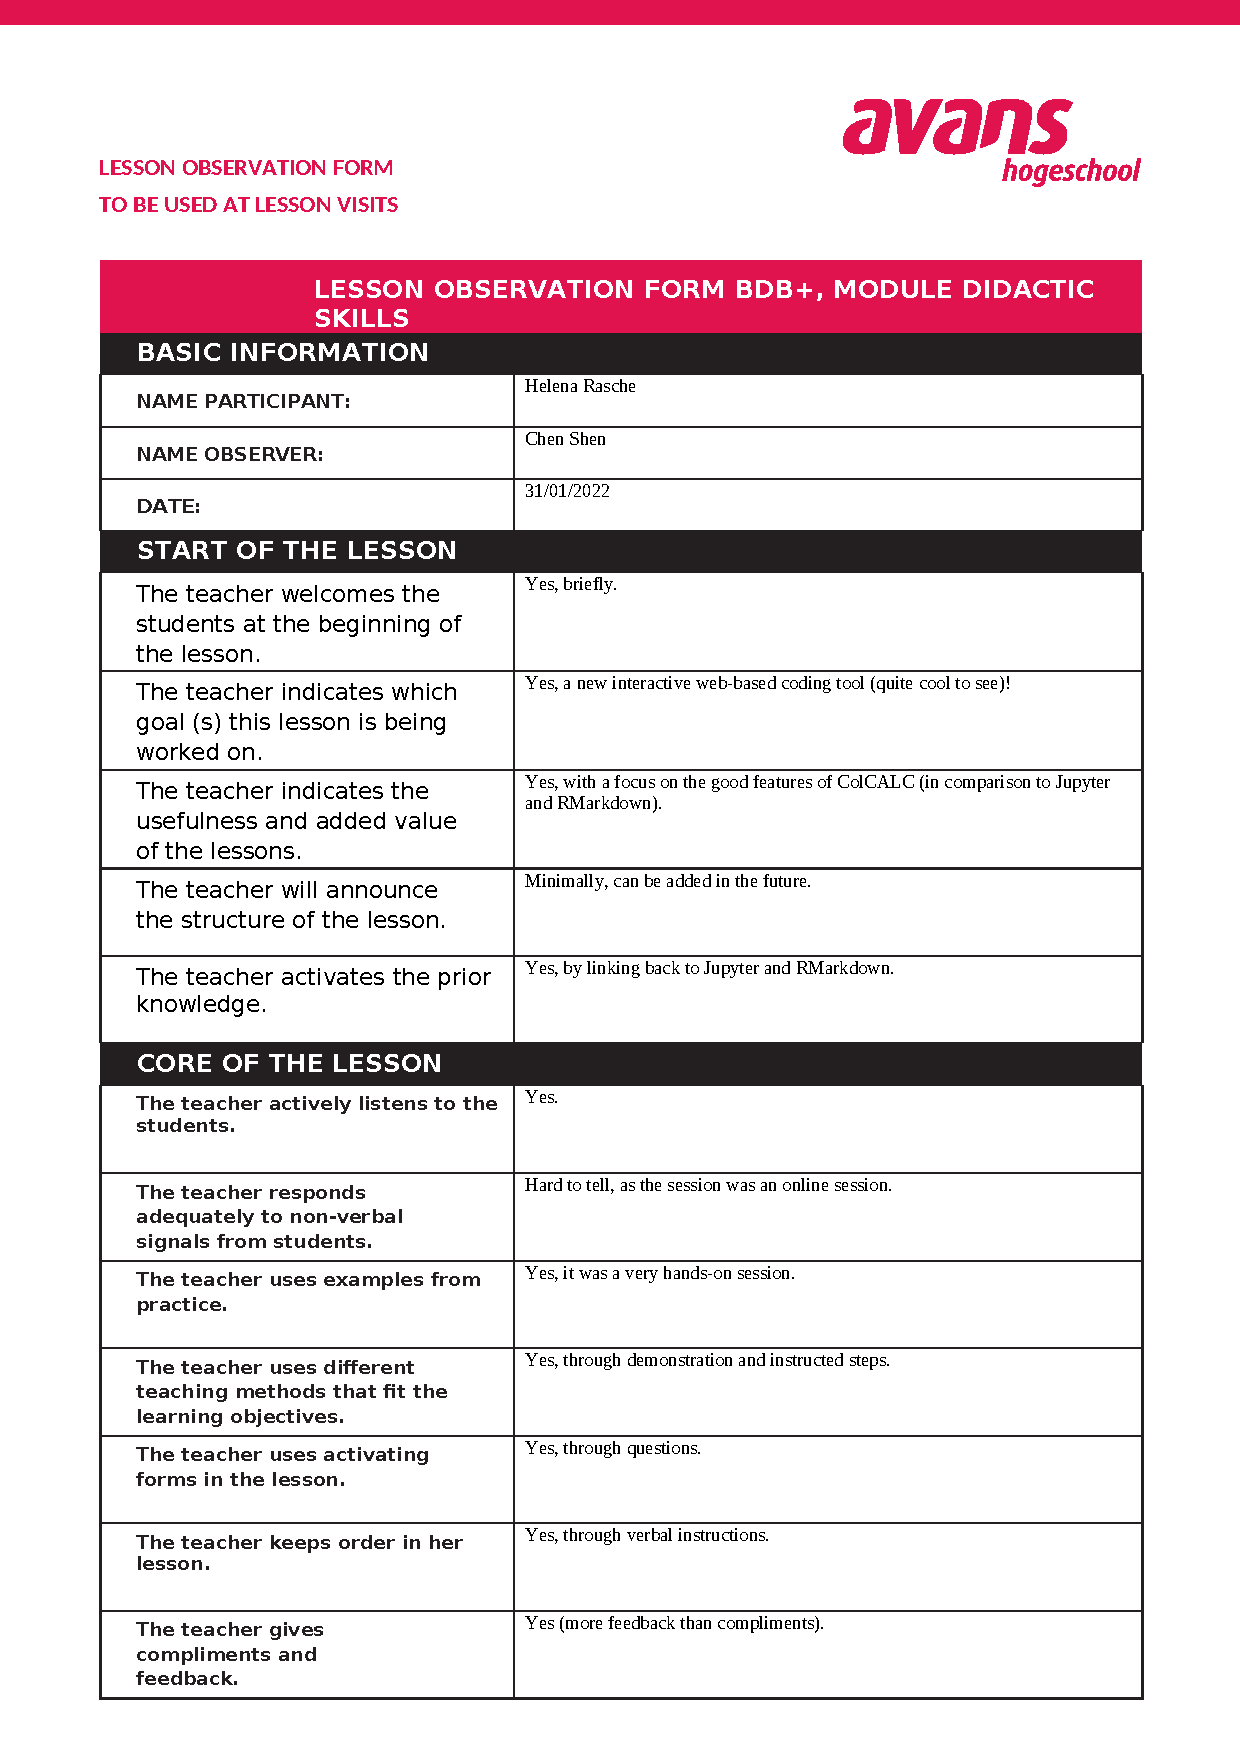
\includepdf[pages=-]{1819 Lesson observation form_Filled_by_Chen_for_Helena.pdf}
\addcontentsline{toc}{section}{Titia for Helena}
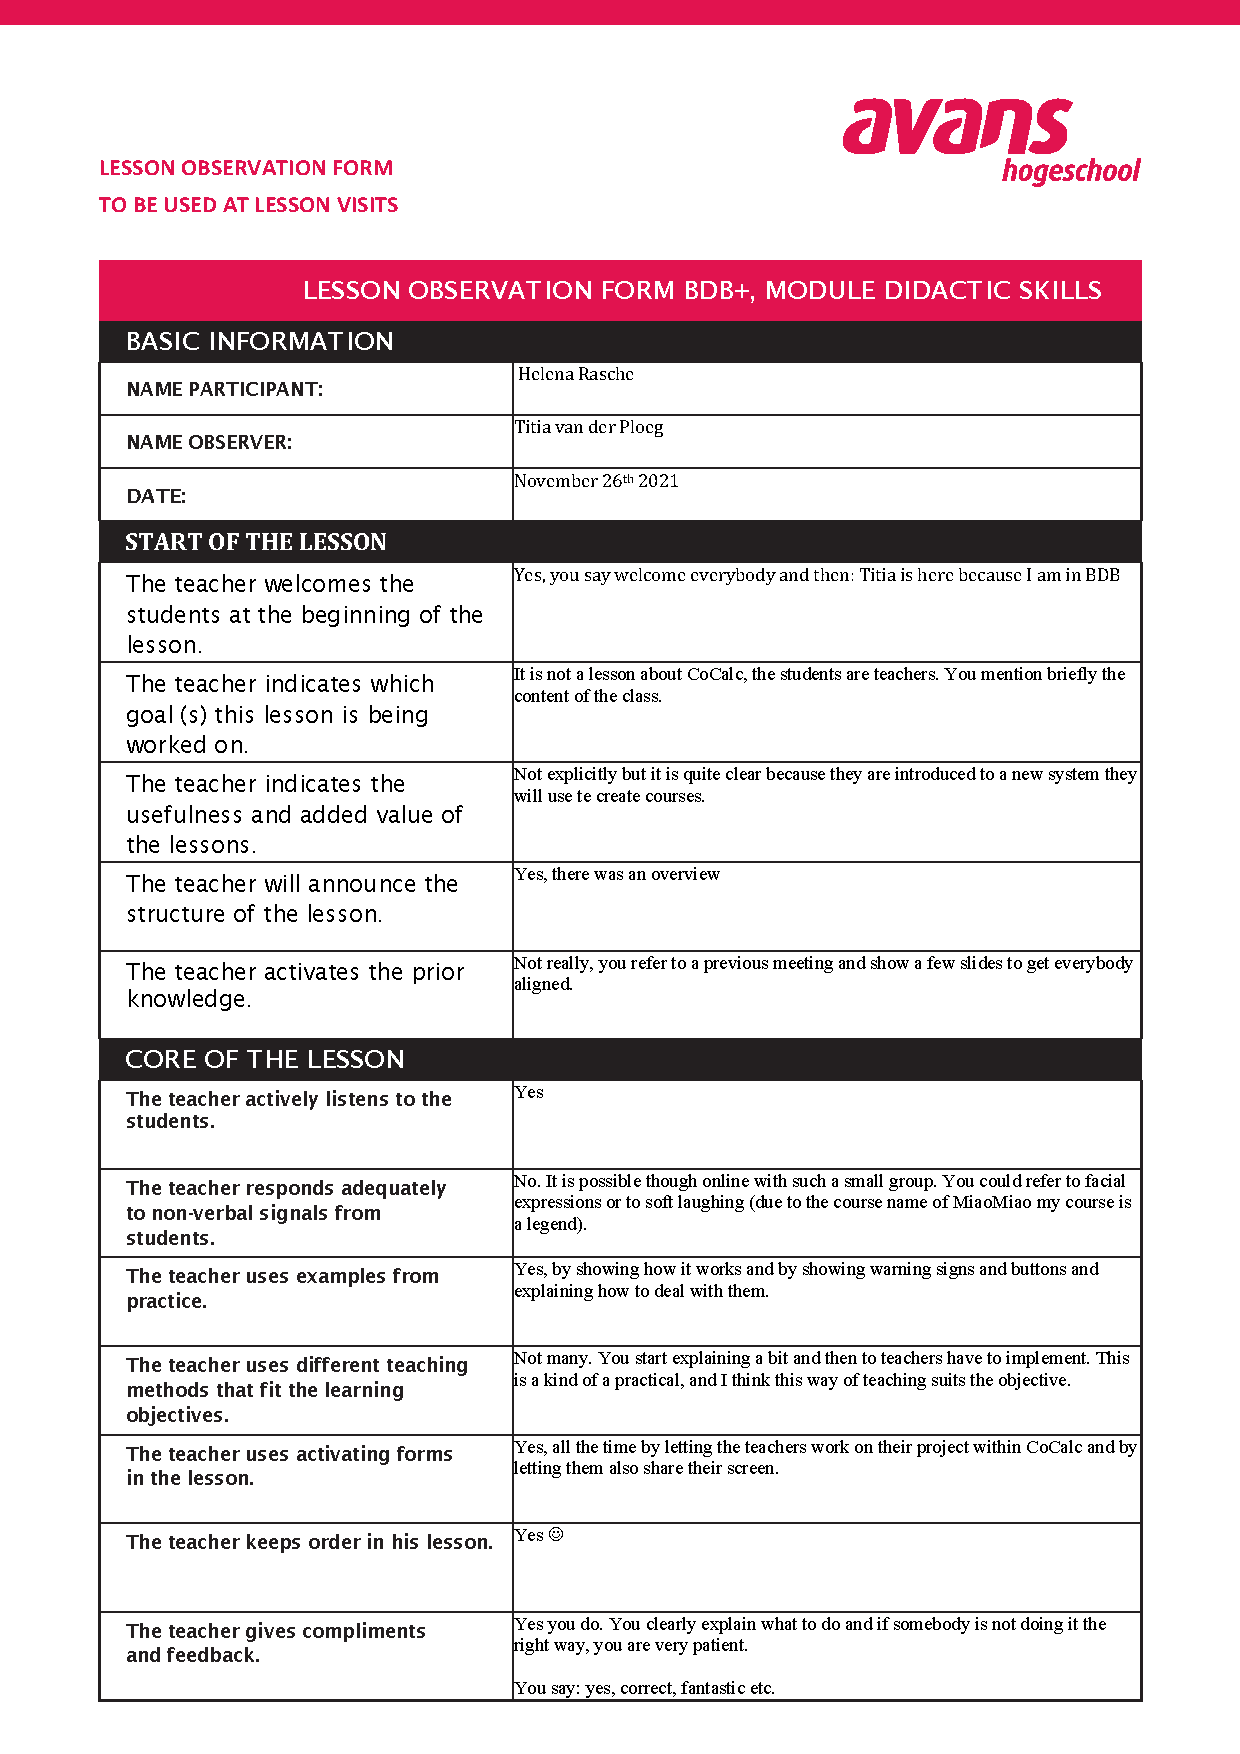
\includepdf[pages=-]{Lesson observation Helena Rasche by TItia 24 nov.pdf}
\addcontentsline{toc}{section}{Helena for Chen}
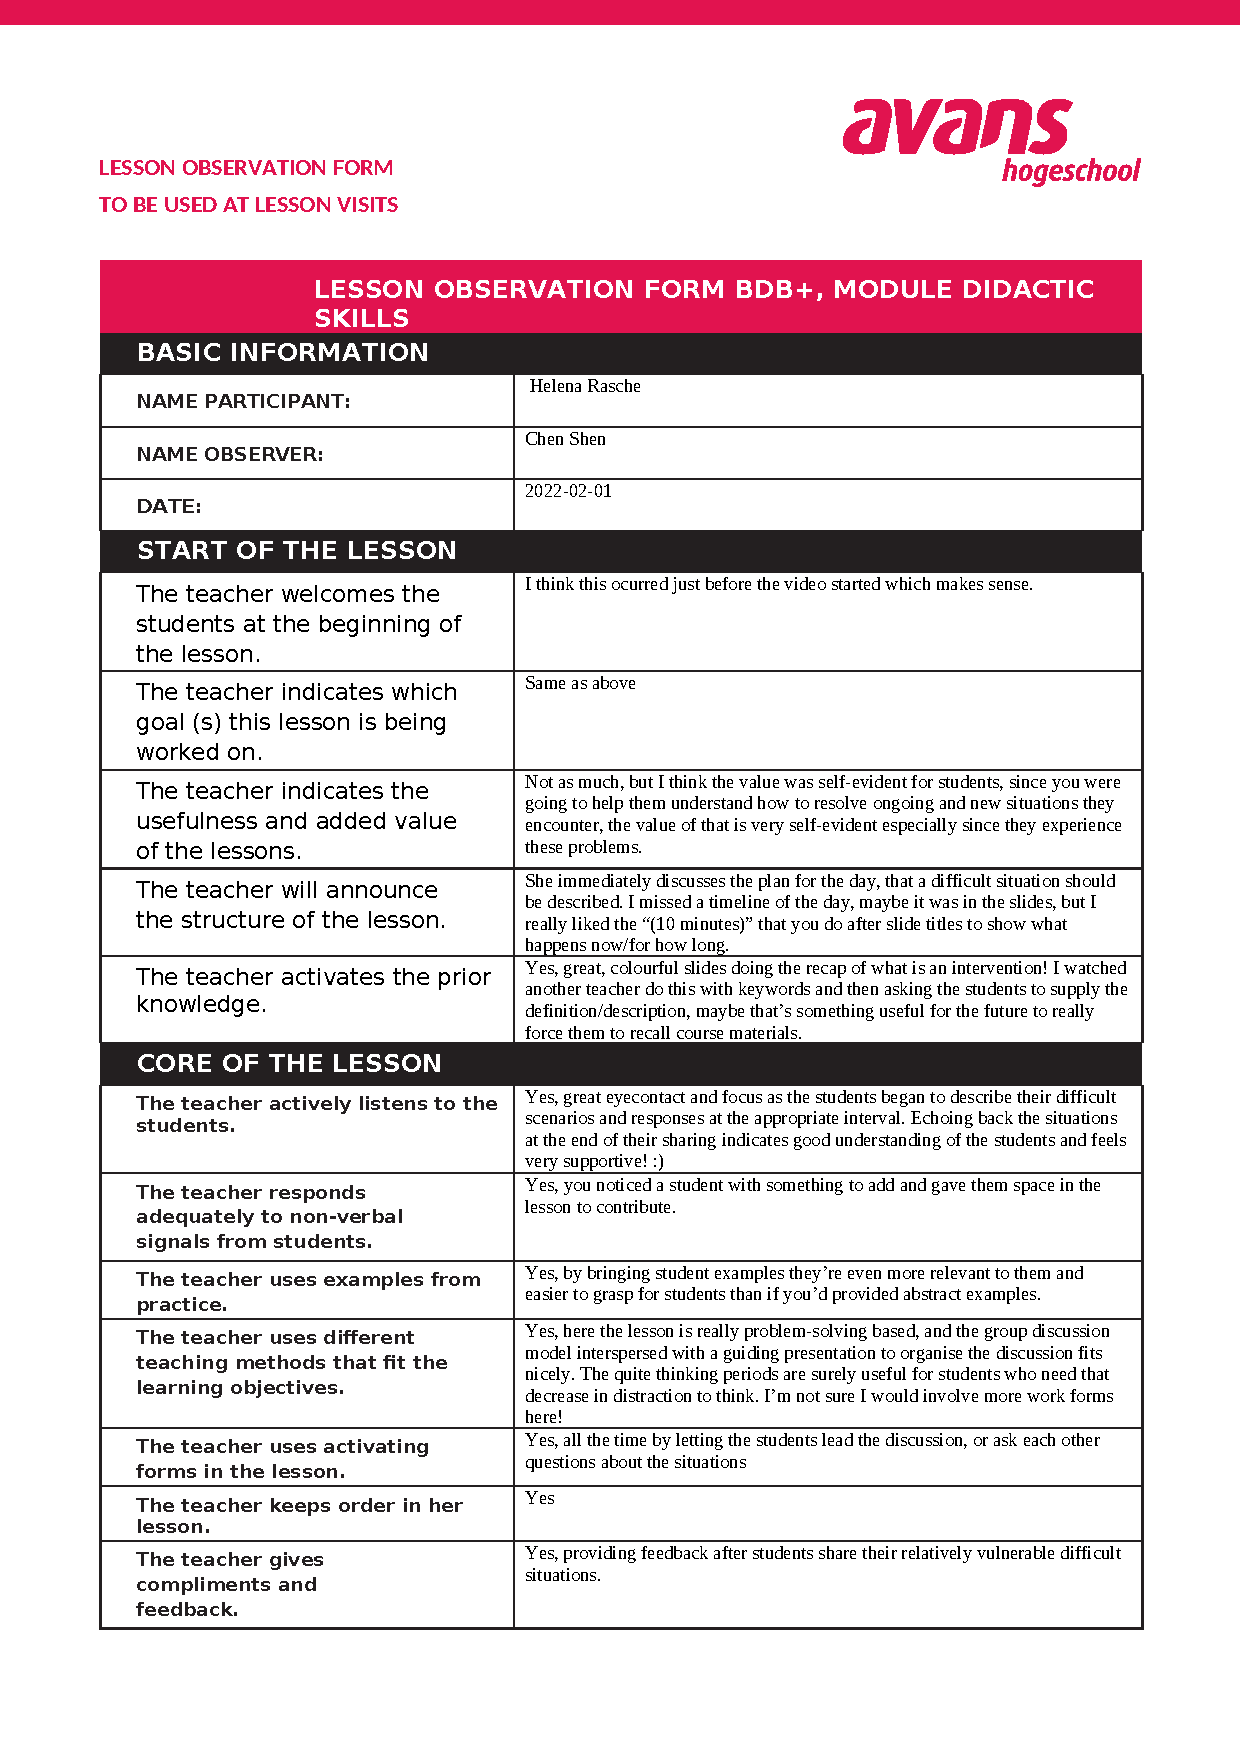
\includepdf[pages=-]{Lesson observation form-1 - for Chen Shen.pdf}
\end{document}
